\documentclass[11pt]{amsbook}

\usepackage{../HBSuerDemir}

\begin{document}


% ++++++++++++++++++++++++++++++++++++++
\hPage{b2p2/317}
% ++++++++++++++++++++++++++++++++++++++

A family (1) dependent on a single parameter admits in general an envelope, 
and the equation of the envelope is given in the theorem:

\begin{thm}
 
 If the family
 
 \[
  \Gamma_{\lambda} : F( x , y , \lambda ) = 0 \tag{1}
 \]
 
 depending on a single parameter $ \lambda $ admits an envelope $ e $, 
 the characteristic point $ C $ of $ \Gamma_{\lambda} $
 satisfies the simultaneous equation
 
 \[
  e: F( x , y , \lambda ) = 0
  \quad , \quad
  F_{\lambda}( x , y , \lambda ) = 0
 \]
 
\end{thm}


\begin{proof}
 
 Each curve $ \Gamma_{\lambda} $ has at least one point of contact with the envelope (characteristic point).
 Let $ C_{\lambda} $ be one of these.
 The coordinates of $ C_{\lambda} $ depend on $ \lambda $
 and verify $ F( x , y , \lambda ) = 0 $ identically.

 \begin{figure}[h]
   \begin{center}
     \includegraphics[scale=0.45]{images/b2p2-317-fig01.png}
   \end{center}
 \end{figure}
 
 Let us express tangency of $ \Gamma_{\lambda} $ and the envelope,
 at $ C_{\lambda} $ :

 Slope of $ \Gamma_{\lambda} $ at $ C_{\lambda} $
 \quad : \quad
 $ -F_{x} / F_{y} $
 
 Slope of $ \,\, e \,\, $ at $C_{\lambda} $
 \quad : \quad
 $ ( \hDif y / \hDif \lambda ) / ( \hDif x / \hDif y ) = 0 $
 
 \[  
  \Rightarrow \quad
  - \frac{ F_{x} }{ F_{y} } = \frac{ \hDif y / \hDif \lambda }{ \hDif x / \hDif \lambda }  
  \quad
  \Rightarrow \quad
  F_{x} \frac{ \hDif x }{ \hDif \lambda } + F_{y} \frac{ \hDif y }{ \hDif \lambda } = 0  
 \]
 
 
 Using this result in the total derivative of
 $ F( x , y , \lambda ) $ with respect to $ \lambda $, we have
 
 \[
  \underbrace{ F_{x} \frac{ \hDif x }{ \hDif \lambda } + F_{y} \frac{ \hDif y }{ \hDif \lambda } }_{0} + F_{\lambda} = 0
  \quad \Rightarrow \quad
  F_{\lambda} = 0.
 \]
 
\end{proof}


\begin{exmp}
 
 Find the envelope of the family of circles of constant radii $ r $, centers on $ x-axis $.
 
\end{exmp}


\end{document}